
\chapter{Testen und Validieren}
\label{chapter_Testen_und_Validieren}

Da das System in einem Langzeit-Teststand eingesetzt wird, ist die Zuverlässigkeit und die Betriebsfähigkeit über lange Zeiträume besonders wichtig. Es darf keine großen Performanceeinbußen oder lange Ausfälle beim Betrieb geben. In diesem Kapitel wird auf die Tests zur Sicherstellung dieser Kriterien und die Grenzen des Systems eingegangen.

\section{Speicherverwaltung}

Ein häufiger Grund für Performanceeinbußen sind Fehler in der Speicherverwaltung. Meist treten dabei Speicherlecks (englisch: memory leak) auf.  Speicherlecks sind Fehler in der Programmierung der Speicherverwaltung, wodurch Speicher belegt, aber ungenutzt ist und nicht wieder freigegeben wird. Dabei kommt es zu einer immer größer werdenden Speichernutzung, bis der gesamte Speicher des Systems ausgelastet ist und es sich stark verlangsamt oder sogar abstürzt.\\
Bei normalen Mikrocontrollern wird die Speicherverwaltung komplett vom Programmierer umgesetzt. Beim BeagleBone Black  übernimmt das Linux-Betriebssystem einen großen Teil der Verwaltung. Jedoch kann es trotzdem noch zu Speicherlecks kommen. Der Hauptgrund ist auf dem Heap durch \textit{malloc()} oder \textit{new} reservierter Speicher der nicht wieder durch \textit{free()} oder \textit{delete} freigegeben wird.\ 
  
Um Speicherlecks auszuschließen wird die Steuerungssoftware mittels Valgrind \cite{valgrind} auf Speicherfehler überprüft. Valgrind ist ein Programm zu Speicherdiagnose. Es ist im Grunde eine virtuelle Maschine, in der das zu testende Programm ausgeführt wird. So läuft das zu testende Programm niemals auf der realen CPU, sondern lediglich in Valgrind. Dadurch können alle Aufrufe und Aktionen eines Programmes überwacht werden. Aus diesen Daten ermittelt Valgrind, ob Speicherfehler vorliegen.\\
Bei der Überprüfung der Steuerungssoftware kommt es lediglich zu einigen falsch positiven (englisch: false positive) Ergebnissen. Sie sind auf die Beschaffenheit der Qt C++ Klassenbibliothek zurückzuführen und können ignoriert werden. Somit kann davon ausgegangen werden, dass die Steuerungssoftware keine Fehler in der Speicherverwaltung aufweist.\\

\section{Fehlerfälle}
Ein Fehlerfall ist der Stromausfall. Nach einem Stromausfall muss das System binnen kürzester Zeit wieder einsatzbereit sein. Zur Sicherstellung dieser Eigenschaft wurden 20 Stromausfälle durch trennen und anschließendes neu verbinden der Stromversorgung simuliert. Bei 20 Versuchen ist das System ohne Probleme neu gestartet. Das BeagleBone Black fährt bei Anschluss einer Stromversorgung automatisch hoch. Auch die Uhrzeit und das Datum werden durch den Einsatz des RTC Capes beibehalten.\ 

Ein weiteres Szenario, ist das Abziehen eines Mess-Slaves im laufenden Betrieb. Der Mess-Server erkennt diesen Fehlerfall und teilt den Fehler über die Benutzeroberfläche dem Administrator mit. Der Mess-Server versucht weiterhin den Mess-Slave in regelmäßigen Abständen zu erreichen. Der Versuch der Kontaktaufnahme erfolgt so lange, bis der Mess-Slave durch das Löschen der RS232 Adresse aus der Datenbank vom System abgemeldet , oder der Mess-Slave wieder angeschlossen wird und somit erreichbar ist. In diesem Fall werden wieder Messdaten in den konfigurierten Intervallen erfasst.

\section{Testaufbau}

\begin{figure}[H]
\begin{center}
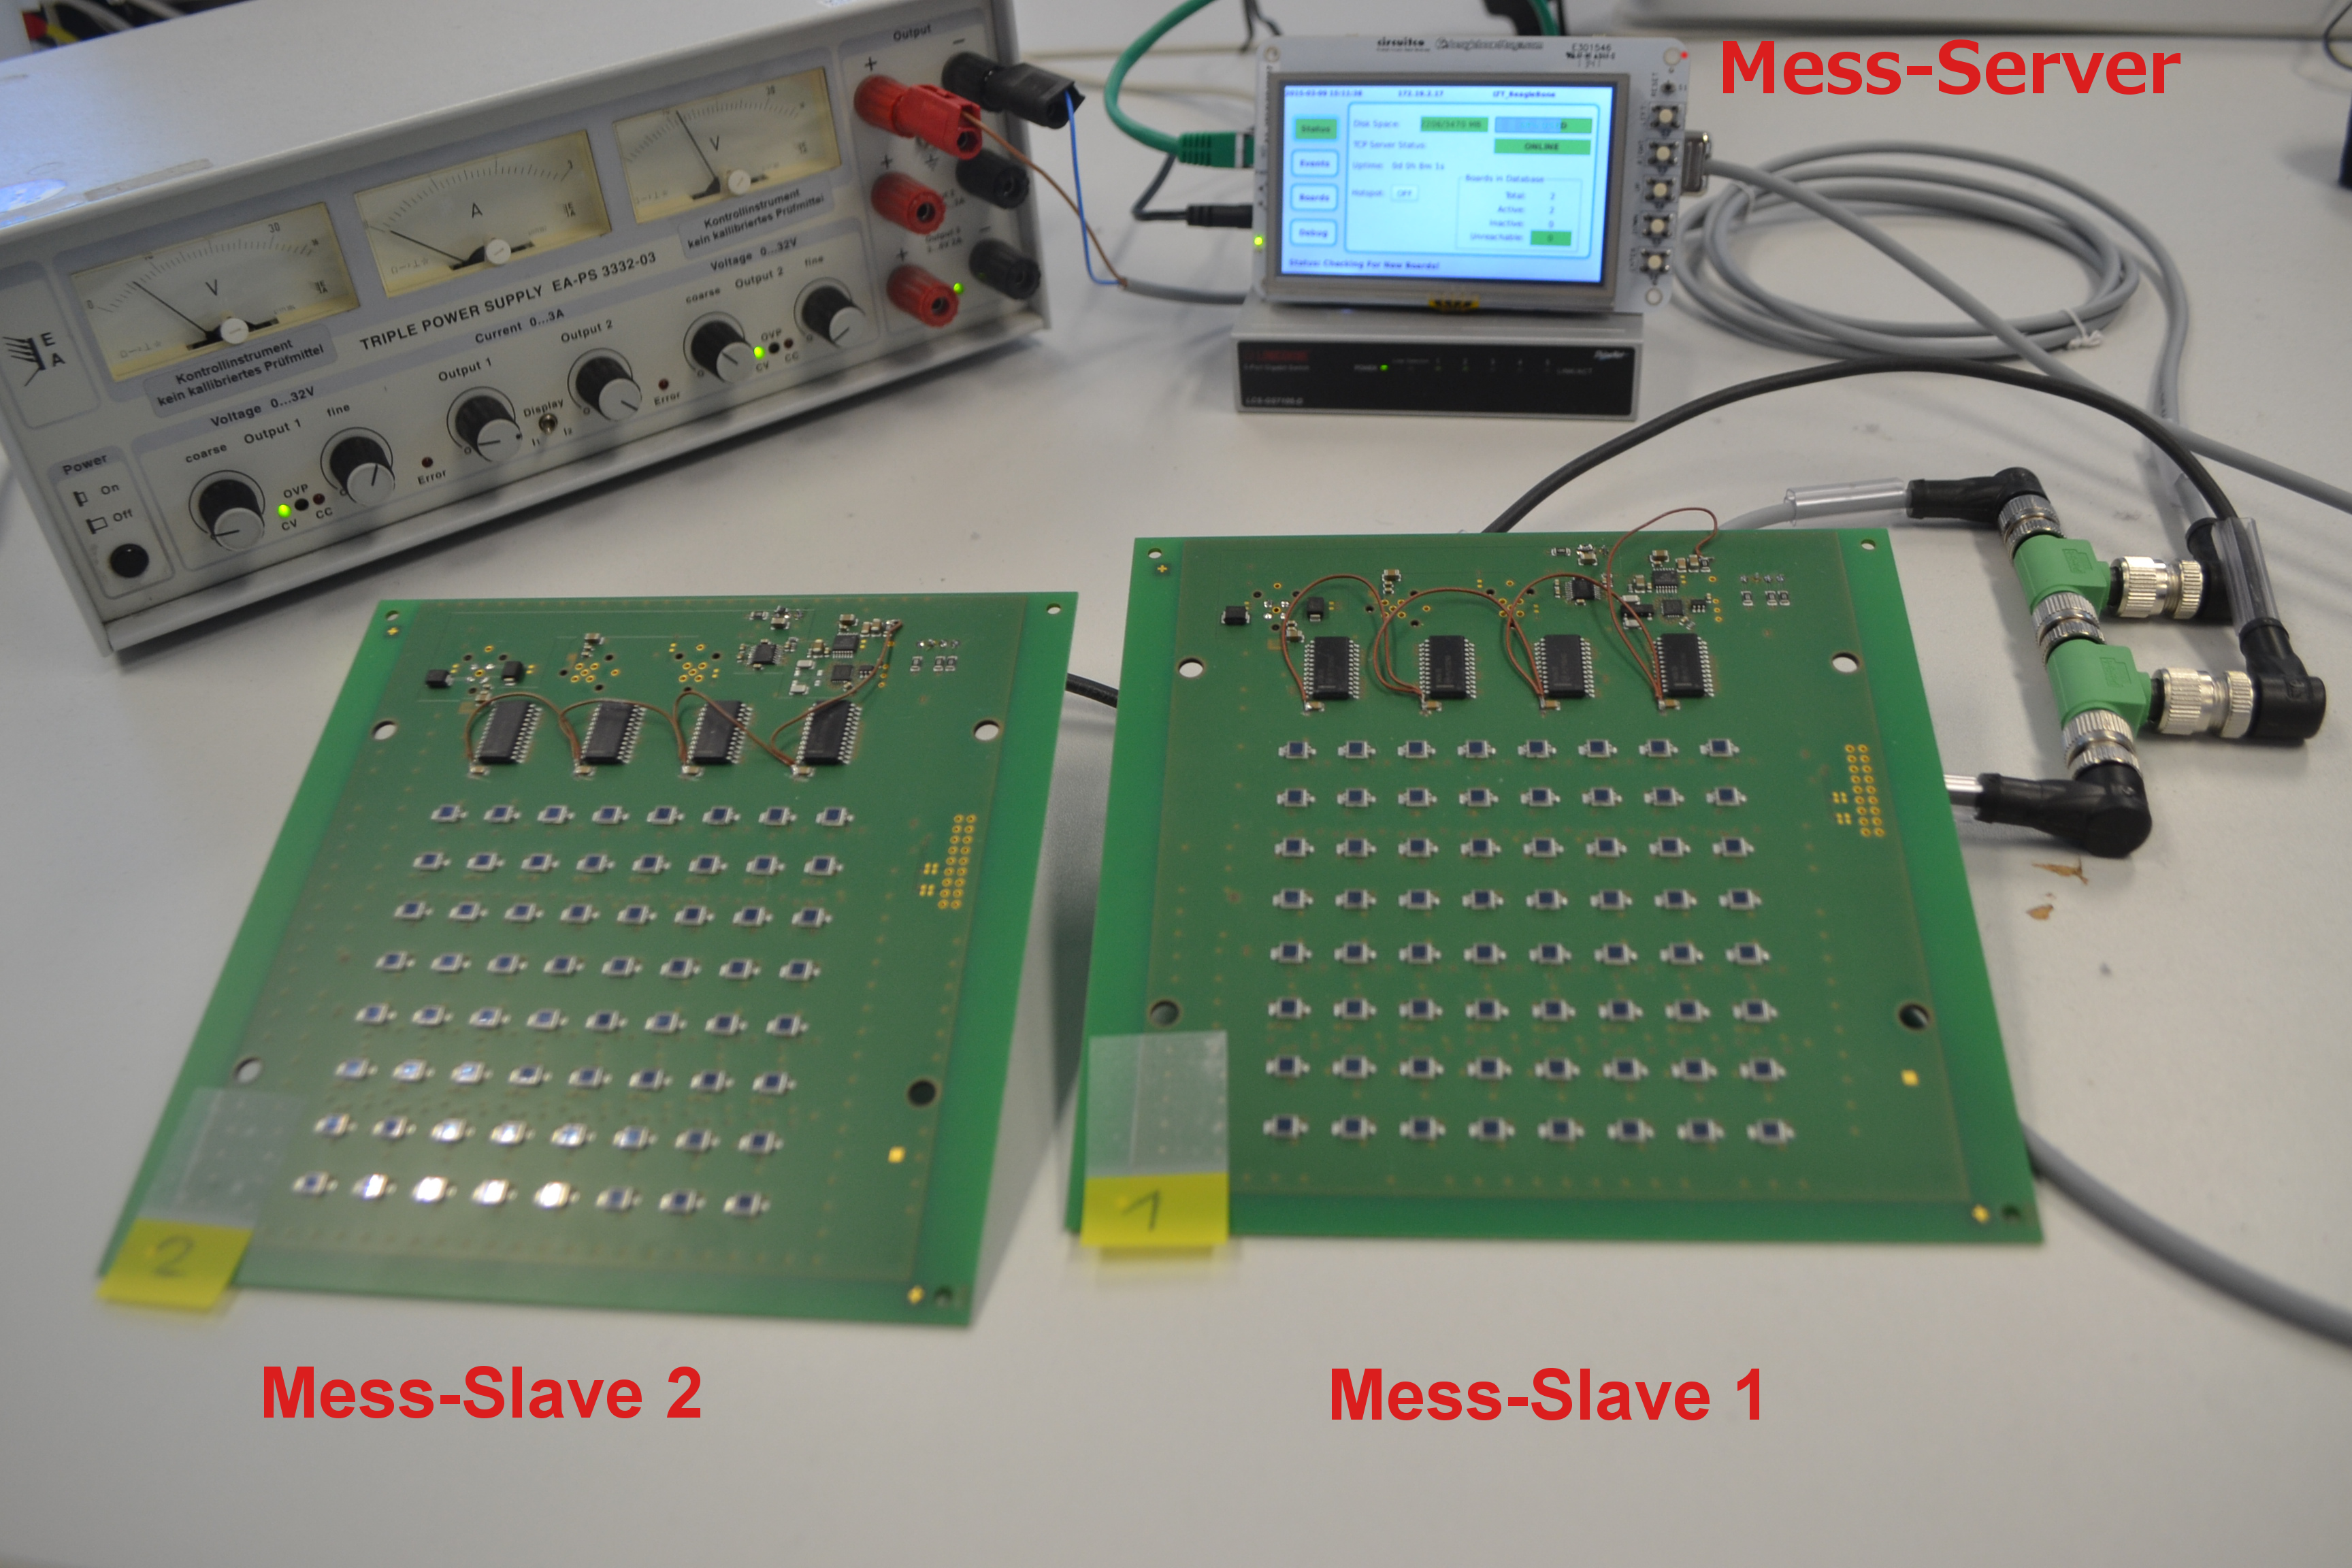
\includegraphics[width=0.7\textwidth]{img/general/Testaufbau.png}
\caption{Testaufbau}
\label{figure_Testaufbau}
\end{center}
\end{figure}

In einem Testaufbau werden zwei Mess-Slaves an einen Mess-Server angeschlossen und in Betrieb genommen. \\
Beiden Mess-Slaves wurde vorher die RS232 Adresse 0 zugewiesen, damit sie sich bei dem Mess-Server anmelden können. Außerdem soll eine Messung pro Stunde durchgeführt werden. Die Mess-Slaves werden nach einander an den RS232 Bus angeschlossen und vom Mess-Server erkannt. Es ist dabei wichtig, zu warten bis der erste Mess-Slave erfolgreich angemeldet ist, bevor der zweite Mess-Slave angeschlossen ist. Würden beide Mess-Slaves gleichzeitig angeschlossen werden, gebe es einen Adresskonflikt, da beide Mess-Slaves die RS232 Adresse 0 besitzen. Es wäre keine Kommunikation möglich.\\
Nach der erfolgreichen Anmeldung am Mess-Server, werden in den eingestellten Messintervallen die Messdaten aufgezeichnet. Über Desktop-Anwendung des PC-Clients kann auf die Mess-Slaves zugegriffen werden. Die Performance des Mess-Servers wird dabei nach durchgängigem Betrieb über 10 Tage nicht beeinflusst. 

\section{Grenzen}

In der Theorie können 127 Mess-Slaves gleichzeitig an einem Mess-Server betrieben werden. Diese Grenze wird durch den RS232 Adressraum gegeben. Jedoch ergeben sich in der Praxis einige Einschränkungen. Die durchschnittliche Dauer für die Erfassung der Messdaten für einen Mess-Slave beträgt 4,64 Sekunden. Dieser Wert wurde aus 25 Messungen gemittelt.\\
Wenn 127 Mess-Slaves angeschlossen sind und für jeden eine Messungen durchgeführt werden soll, ergibt sich folgende Zeit für einen gesamten Durchlauf.\ 

\newpage
\begin{center}
{\large$AnzahlDerMessSlaves * DauerProMessung = Durchlaufzeit$}\ 


{\large$127 * 4,64 s = 589,28 s$}
\end{center}\ 

Das bedeutet, dass bei 127 Mess-Slaves das minimal Messintervall 589 Sekunden beträgt.\ 

Der typische Betrieb eines Mess-Slaves sieht ca. 365 Messungen pro Jahr vor. Bei 64 Prüfobjekten ergibt das 23.360 Messwerte in einem Jahr. Bei zwei Millionen Messwerten in der Datenbank, wird diese in der Performance spürbar negativ beeinflusst. Eine typische Abfrage dauert so bei zwei Millionen Einträgen bereits bis zu fünf Sekunden, im Vergleich zu 160 Millisekunden bei 35 Tausend Einträgen. Nehme man diese 2 Millionen als obere Grenze ergibt sich folgende maximale Anzahl von Betriebsjahren.

\ 
\begin{center}
{\large$MaxMesseinträge / MessungenProJahr = MaxBetriebsjahre$}\ 


{\large$2.000.000 / 23360 = 85,6$}
\end{center}
Jedes Prüfobjekt soll für 20.000 Stunden getestet werden, was 2,28 Jahren entspricht. Daraus kann die maximale Anzahl an Mess-Slaves ermittelt werden.\ 

\ 
\begin{center}
{\large$MaxBetriebsjahre / MessDauer = AnzahlAnMessSlaves$}\ 


{\large$88,6 / 2,28 = 37,5$}
\end{center}\ 

Es ergibt sich eine maximale Anzahl von 37 Slaves pro Mess-Server. Nach 37 abgeschlossenen Langzeittests muss durch den Administrator alte Messdaten gelöscht werden um Raum für neue zu schaffen.\ 

In der Praxis wird pro Temperaturschrank ein Mess-Server eingesetzt. In jedem dieser Temperaturschränke können bis zu zehn Mess-Slaves gleichzeitig betrieben werden. Daraus ergibt sich eine Betriebsdauer von 8,86 Jahren, bevor von einem Administrator in das System eingegriffen werden muss.